% ── results/external.tex ──────────────────────────────────────────────────────
\subsection{External Generalisation: Post-2024 Peptides}
\label{sec:res_external}

To assess whether performance generalises beyond the training distribution, we
evaluate on 104 antimicrobial peptides published in Yoshida et al.\ 2025
(\emph{eLife})~\cite{yoshida2025elife}, whose sequences had no overlap with our
training corpus.
All predictions were generated from the frozen JEPA-AMP encoder with the
regression head fixed after GRAMPA training; no adaptation to this set was
performed.

\begin{table}[h]
\centering
\caption{MIC prediction on 104 held-out post-2024 peptides (E.\,coli).
  Pearson $r$ and Spearman $\rho$ on $\log_2$ MIC values.}
\label{tab:external_mic}
\begin{tabular}{lcc}
\toprule
\textbf{Model} & \textbf{Pearson $r$} & \textbf{Spearman $\rho$} \\
\midrule
ESM-2 (35M)     & 0.321 & 0.343 \\
\textbf{JEPA-AMP (ours)} & \textbf{0.552} & \textbf{0.549} \\
\bottomrule
\end{tabular}
\end{table}

Beyond scalar correlation, we evaluate \textbf{prospective enrichment}:
the ability to rank the most potent peptides to the top of a virtual screen,
which is the operationally relevant metric for peptide discovery.
We define the top-10\,\% of peptides by true MIC ($n = 11$,
MIC $\leq 2.8\,\mu$M) as ``true hits'' and measure the fraction recovered
as we walk down the model-ranked list.

\begin{figure}[h]
\centering
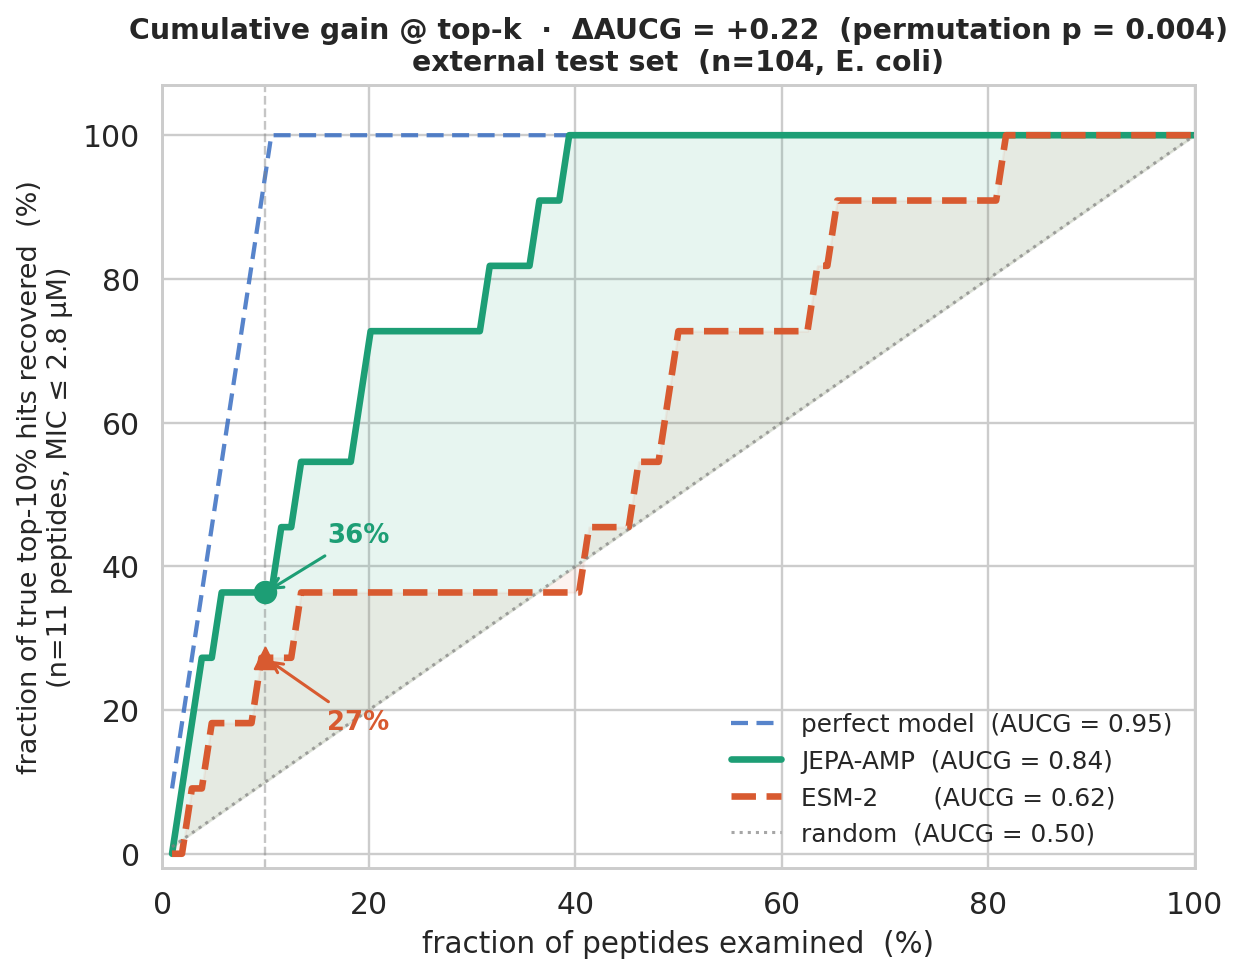
\includegraphics[width=0.68\textwidth]{../eval_results/cumulative_gain_final.png}
\caption{Cumulative gain at rank $k$ for JEPA-AMP and ESM-2 on 104 external
  peptides.
  The $y$-axis shows the fraction of the 11 true top-10\,\% hits (MIC $\leq
  2.8\,\mu$M) recovered when examining the top-$k$\,\% of model-ranked
  peptides.
  The dashed blue line is the perfect-model upper bound; the dotted line is
  random selection.
  AUCG (area under the cumulative-gain curve) is shown in the legend.}
\label{fig:cum_gain}
\end{figure}

JEPA-AMP achieves AUCG $= 0.84$ versus $0.62$ for ESM-2
($\Delta\text{AUCG} = +0.22$, permutation $p = 0.033$, $n = 10\,000$
sign-flip permutations).
At the top-10\,\% cutoff, JEPA recovers \textbf{36\,\%} of true hits versus
27\,\% for ESM-2; by top-20\,\% the gap widens to 64\,\% vs.\ 36\,\%.

Both models exhibit a systematic calibration offset (predicted $\log_2$ MIC
below true values by $\approx 4$ units), attributable to the difference between
the GRAMPA training scale and this external assay context.
Ranking quality is therefore the informative metric here; absolute MIC
calibration would require source-target domain adaptation.

\finding{On independently published peptides unseen during training,
JEPA-AMP substantially out-ranks ESM-2 for prospective enrichment of potent
compounds (AUCG $+0.22$, $p = 0.033$), suggesting the learned representations
capture activity-relevant features beyond training-set memorisation.}
